%----------------------------------------------------------------------------
\chapter{Jegyzőkönyv}
%----------------------------------------------------------------------------





%----------------------------------------------------------------------------
\section{A labor témája}
%----------------------------------------------------------------------------
A mérés során egy sorompó irányítását terveztük meg, melyet a diszkrét eseményű rendszerek felügyeleti irányításával valósítottunk meg. A modellt és annak specifikációit a Supremica programban alkottuk meg, majd azt a Matlab Stateflow bővítményének segítségével teszteltük.


%----------------------------------------------------------------------------
\section{Szabályozandó szakasz megtervezése}
%----------------------------------------------------------------------------
A sorompót mozgató motor modellje a \figref{Motor}~ábrán látható. Három állapota lehet, vagy fel-, vagy lemozgatja a sorompó rudat, vagy egy helyben tartja azt. 

\begin{figure}
	\centering
	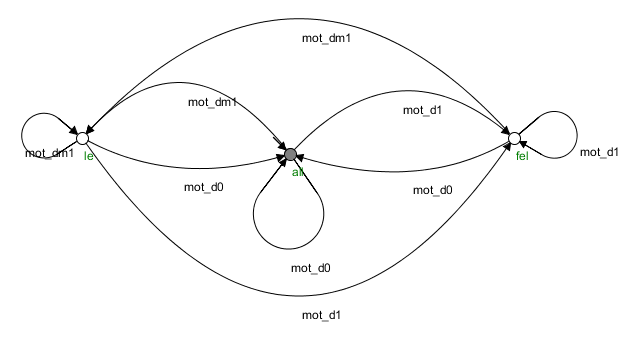
\includegraphics[width=110mm,keepaspectratio]{figures/2m03/b_motor.png}
	\caption{A sorompó rúd mozgató motor modellje}
	\label{fig:Motor}
\end{figure}
Ezen állapotok között a következő eseményekkel lehet váltani:
\begin{itemize}
	\item \textbf{mot\_d1} - Sorompó felfelé indítása
	\item \textbf{mot\_dm1} - Sorompó lefelé indítása
	\item \textbf{mot\_d0} - Sorompó megállítása
\end{itemize}
Mint látható, ezen modell megengedi, hogy a mozgás közben ismételten ráindítsunk a motorra, álló helyzetben ismét leállítsuk vagy akár ellentétes irányú ráindítás is lehetséges, mely a motor élettartamát jelentősen csökkentené. Ezen jelenségek letiltása miatt egy specifikációt vezettünk be, mely a \figref{SpecMot}~ábrán látható.

\begin{figure}
	\centering
	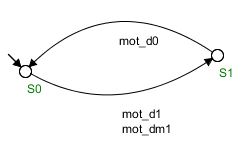
\includegraphics[keepaspectratio]{figures/2m03/b_spec_motor.png}
	\caption{A mozgató motor specifikációja}
	\label{fig:SpecMot}
\end{figure}
A Supremica \textit{Analyzer} fülén az eddig megvalósított automaták szinkron szorzatát a \textit{Synchronize} paranccsal valósítottuk meg, az így készült modell (továbbiakban \textit{sup\_mot}) -mely már megfelel a specifikációnak- a \figref{SupMot}~ábrán látható.
\begin{figure}
	\centering
	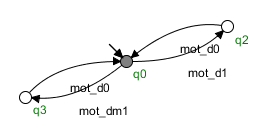
\includegraphics[keepaspectratio]{figures/2m03/b_supmot.png}
	\caption{A mozgató motor végleges modellje}
	\label{fig:SupMot}
\end{figure}


\newpage
%----------------------------------------------------------------------------
\section{A végálláskapcsoló és fizikai korlátok}
%----------------------------------------------------------------------------
A motor helyes vezérléséhez szükségünk lesz egy-egy végálláskapcsolóra, mely a legfelső (\textit{top\_}), illetve legalsó (\textit{bottom\_}) helyzet elérését jelzik, vagyis a motor megállítására figyelmeztetnek. Eddig a modellben csak általunk irányítható eseményeket vettünk fel, ám a végálláskapcsoló jelzésének idejét nem tudjuk kontrollálni, ezt külön meg kell jelölnünk a Supremicában. Mindkét kapcsoló jelének fel, illetve lefutó élére következik be esemény, ezeket a \textit{rise} és \textit{fall} címkével jeleztük. A végálláskapcsolókhoz tartozó automata (\figref{Limit}~ábra) kezdeti állapota az, hogy a sorompó az alsó végállásban van. További állapotok, ha két végállás között valahol félúton, vagy a felső végállásban van a sorompó rúd.
\begin{figure}
	\centering
	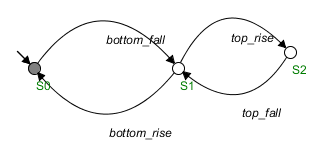
\includegraphics[keepaspectratio]{figures/2m03/b_limit.png}
	\caption{A végálláskapcsolók modellje}
	\label{fig:Limit}
\end{figure}
Mivel nem irányítható eseményeket terveztünk a rendszerbe, így azok jelenleg bármikor bekövetkezhetnek, ám helyes működés esetén ezen eseményeknek fizikai korlátai vannak. Feltételezhetjük, hogy az alsó végálláskapcsoló jelzésének lefutó éle, és a felső kapcsoló jelzésének felfutó éle csak a sorompó felfelé mozgása közben következhet be. Ehhez hasonlóan a \textit{top\_fall}, illetve a \textit{bottom\_rise} esemény csak lefelé mozgás közben történhet. Ezeket a fizikai korlátokat is felvittük a programba, melyek a \figref{Constraints}~ábrán láthatóak.

\begin{figure}
	\centering
	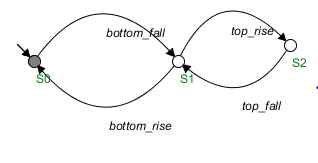
\includegraphics[keepaspectratio]{figures/2m03/b_constraint1.png}	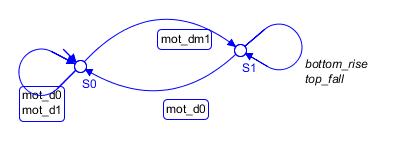
\includegraphics[keepaspectratio]{figures/2m03/b_constraint2.png}
	\caption{A fizikai korlátok modelljei}
	\label{fig:Constraints}
\end{figure}

Az előző pontban taglalt \textit{sup\_mot}, valamint az ebben a pontban megvalósított automaták szinkron szorzatát véve elkészítettük a \textit{barrier} modellt, mely a sorompó mozgatását megvalósító funkciók összesített modellje. Ennek állapotgráfja látható a \figref{Barrier}~ábrán.

\begin{figure}
	\centering
	\includegraphics[trim = 10mm 55mm 50mm 10mm,clip,width=110mm,keepaspectratio]{figures/2m03/barrier2.pdf}
	\caption{A sorompó mozgatását megvalósító funkciók állapotgráfja}
	\label{fig:Barrier}
\end{figure}




%----------------------------------------------------------------------------
\section{Az infraérzékelő és a távirányító}
%----------------------------------------------------------------------------
A sorompó akkor működik jól, ha az nem záródik rá és nem tesz kárt az ügyfél gépjárművében. Ennek megakadályozására infrasugaras érzékelőt használunk, melyet a rendszerbe kell integrálnunk. Továbbá az ügyfél szeretné távirányítóval nyithatóvá tenni a sorompót. E két rendszer modellje látható a \figref{InfraRemote}~ábrán, melyen az infra jel felfutó éle jelzi az akadály megjelenését, illetve a lefutó éle annak eltűnését. A távirányító szempontjából elég nekünk a gomb megnyomását érzékelnünk. Ezen események ismét általunk kontrollálhatatlanok, ezeket jelezni kell a programnak. 

\begin{figure}
	\centering
	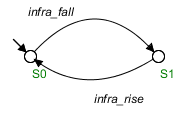
\includegraphics[keepaspectratio]{figures/2m03/b_infra.png}	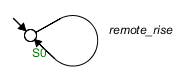
\includegraphics[keepaspectratio]{figures/2m03/b_remote.png}
	\caption{Az infraérzékelő és a távirányító modelljei}
	\label{fig:InfraRemote}
\end{figure}

Az eddig meglévő \textit{barrier}, illetve az újonnan megvalósított két modellt ismét \textit{szinkronizáljuk} a Supremica segítségével, továbbiakban ez lesz a plant, mely a \figref{Plant}~ábrán látható.

\begin{figure}
	\centering
	\includegraphics[trim = 15mm 70mm 50mm 10mm,clip,width=140mm,keepaspectratio]{figures/2m03/plant.pdf}
	\caption{A teljes rendszer működését megvalósító állapotgép}
	\label{fig:Plant}
\end{figure}

%----------------------------------------------------------------------------
\section{Specifikációk}
%----------------------------------------------------------------------------


\newpage
%----------------------------------------------------------------------------
\section{Első feladat}
%----------------------------------------------------------------------------
A mérésvezető által meghatározott {$k_i \in$ [0.9 1.1], $\Theta_i \in$ [0 1]} bizonytalanság és késleltetés mellett inicializáltam a linearizált modellt az \textit{olp\_col} függvénnyel. 

\begin{figure}[!ht]
	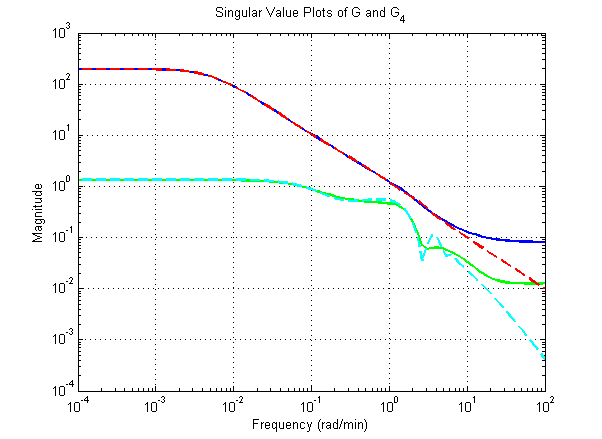
\includegraphics[width=75mm,keepaspectratio]{figures/2m06/olp_old_1_.png}
	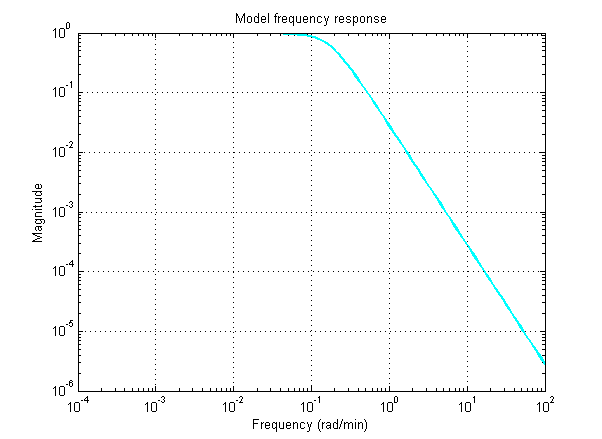
\includegraphics[width=75mm,keepaspectratio]{figures/2m06/olp_old_2_.png}
	\caption{A zárt rendszer frekvencia válasza}
	\label{fig:Init}
\end{figure}

A mérési útmutatóban található súlyozó függvény alapján a \textit{hin\_col} paranccsal megterveztem a szabályzót, mely a \figref{HinOld}~ábrán látható. Ezután leszimuláltam a megadott bizonytalanságok alapján a rendszert, melynek tranziensei a \figref{PrtOld1}~ábrán és a \figref{PrtOld2}~ábrán láthatóak, attól függően, hogy az első vagy a második bemenethez tartozó alapjelre adtunk egységugrást.

\begin{figure}[!ht]\hspace{36mm}
	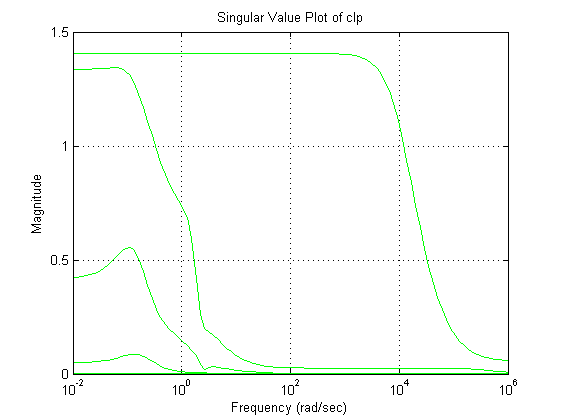
\includegraphics[width=75mm,keepaspectratio]{figures/2m06/hin_old_.png}
		\caption{A megvalósított szabályzó}
	\label{fig:HinOld}
\end{figure}
\begin{figure}[!ht]
	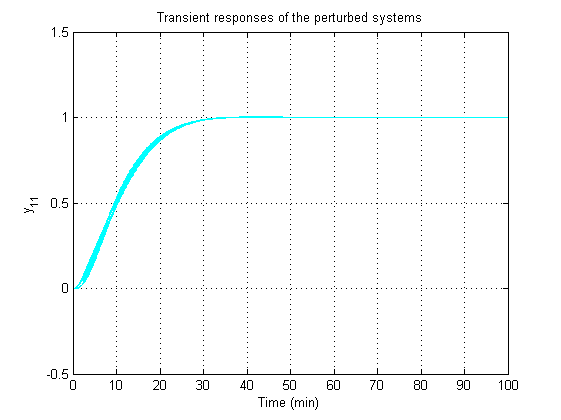
\includegraphics[width=75mm,keepaspectratio]{figures/2m06/prt_old_1.png}
	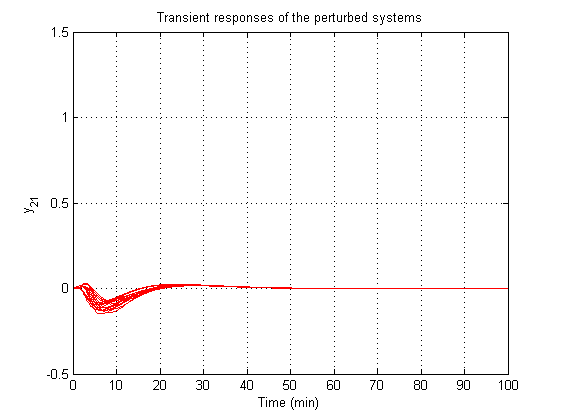
\includegraphics[width=75mm,keepaspectratio]{figures/2m06/prt_old_2.png}\vspace{2mm}
	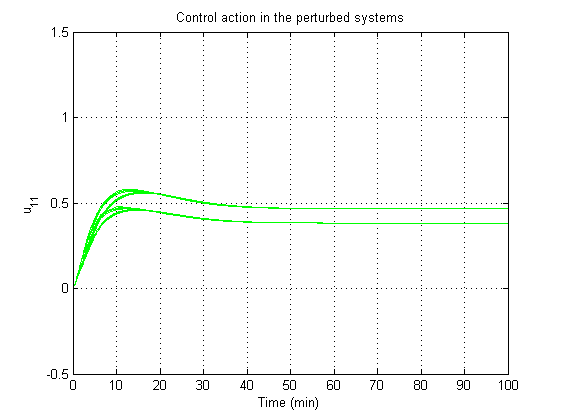
\includegraphics[width=75mm,keepaspectratio]{figures/2m06/prt_old_3.png}
	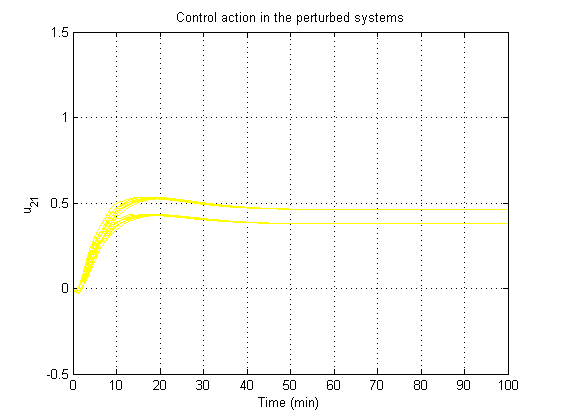
\includegraphics[width=75mm,keepaspectratio]{figures/2m06/prt_old_4.png}
		\caption{A rendszer beavatkozó jelei és kimenetei, az első alapjelhez tartozó egységugrás esetén}
	\label{fig:PrtOld1}
\end{figure}
\begin{figure}[!ht]
	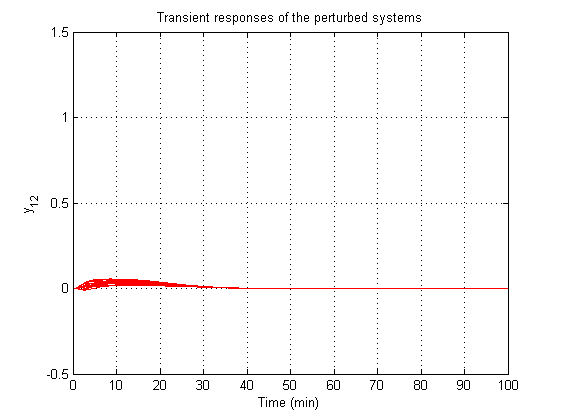
\includegraphics[width=75mm,keepaspectratio]{figures/2m06/prt_old_5.png}
	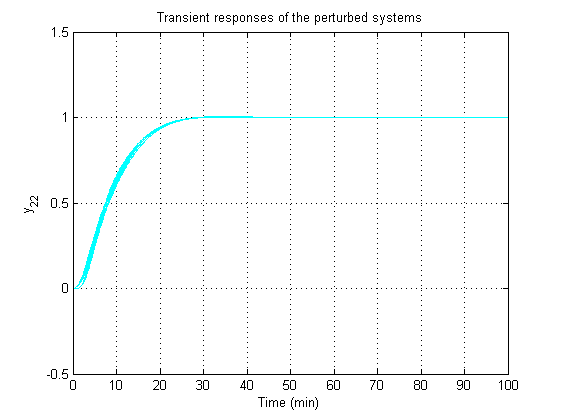
\includegraphics[width=75mm,keepaspectratio]{figures/2m06/prt_old_6.png}\vspace{2mm}
	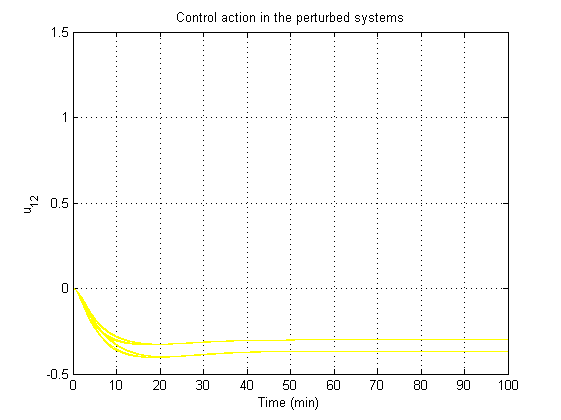
\includegraphics[width=75mm,keepaspectratio]{figures/2m06/prt_old_7.png}
	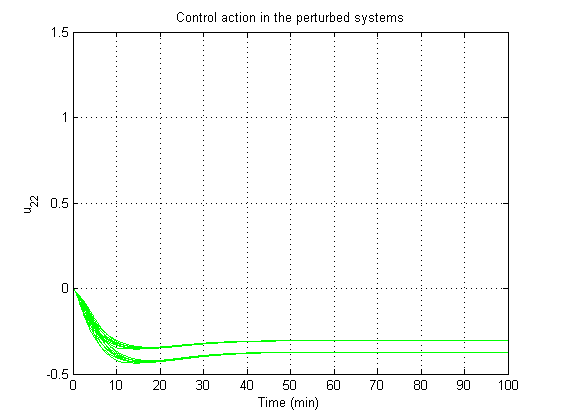
\includegraphics[width=75mm,keepaspectratio]{figures/2m06/prt_old_8.png}
		\caption{A rendszer beavatkozó jelei és kimenetei, a második alapjelhez tartozó egységugrás esetén}
	\label{fig:PrtOld2}
\end{figure}

\newpage
%----------------------------------------------------------------------------
\section{Második feladat}
%----------------------------------------------------------------------------

A rendszer bizonytalanságát növelve az első feladatban megvalósított szabályzó már nem lesz elég robusztus, és elveszti a stabilitását. Erre láthatóak példák a \figref{PrtMod}~ábrán, melyeken az elsőn egy enyhén, a másodikon egy erősen szélesebb bizonytalanságot és késleltetést állítottam be.
A beállított paraméterek értékei:
\begin{itemize}
	\item Enyhébb eset: {$k_i \in$ [0.7 1.3], $\Theta_i \in$ [0 1.07]}
	\item Erősebb eset: {$k_i \in$ [0.65 1.35], $\Theta_i \in$ [0 1.1]}
\end{itemize}

\begin{figure}[!ht]
	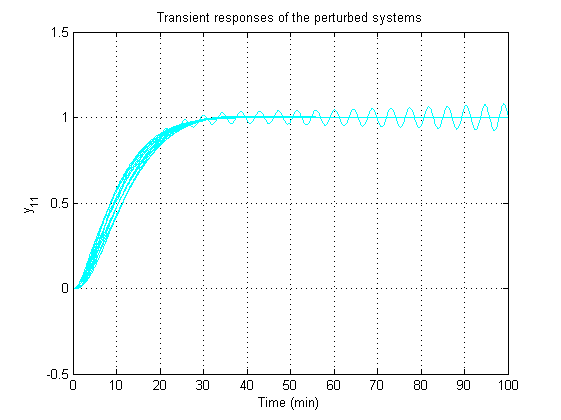
\includegraphics[width=75mm,keepaspectratio]{figures/2m06/prt_small_1.png}
	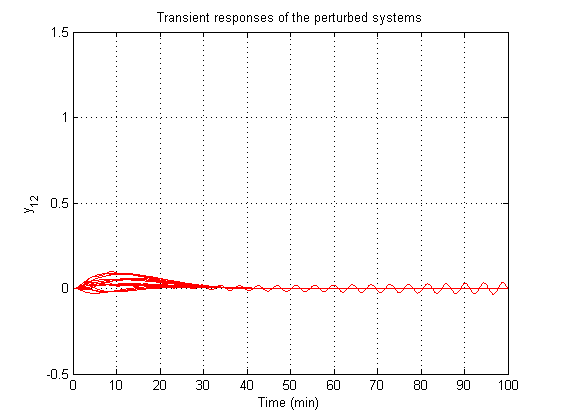
\includegraphics[width=75mm,keepaspectratio]{figures/2m06/prt_small_2.png}\vspace{2mm}
	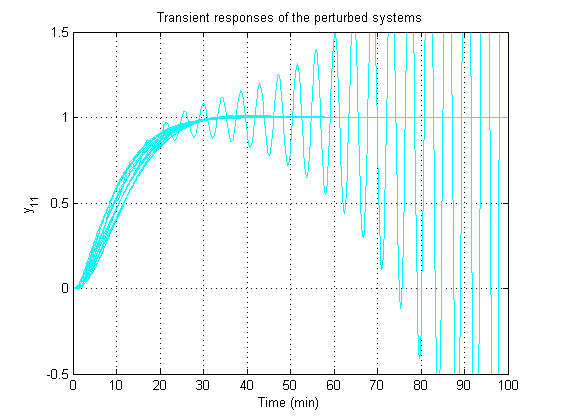
\includegraphics[width=75mm,keepaspectratio]{figures/2m06/prt_big_1.png}
	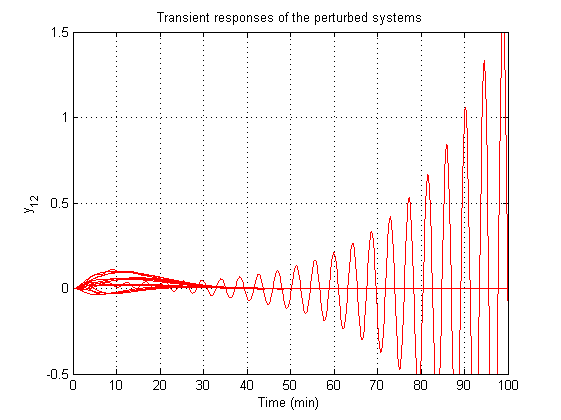
\includegraphics[width=75mm,keepaspectratio]{figures/2m06/prt_big_2.png}
		\caption{A rendszer válaszának tranziensei szélesebb bizonytalanságot feltételezve}
	\label{fig:PrtMod}
\end{figure}

\newpage
%----------------------------------------------------------------------------
\section{Harmadik feladat}
%----------------------------------------------------------------------------
Az új szabályzót az előző feladatban bemutatott, enyhén növelt bizonytalansági feltételek mellett terveztem meg. Ehhez az \textit{unc\_col} függvényt hívtam meg, melyben előzetesen módosítottam a késleltetést és a bizonytalanságot, így az már az új feltételekből kapott görbeseregeket jeleníti meg. A \textit{wfit} parancs segítségével ezekhez új súlyozó függvényt tudtam keresni, mely a következő lett:
\begin{equation}\label{NewWeight}
\frac{2.3509    s^{3}+8.4222   s^{2}+13.6532s+    3.0960}{s^{3}+4.6982  s^{2}+ 10.2369    s+9.4826}
\end{equation}

A \textit{wts\_col} fájlt ezek alapján fel is frissítettem, majd újraszimuláltam a rendszert.


Amint azt a \figref{PrtNew}~ábrán is látni, az új szabályzó a kibővített bizonytalansági feltételek mellett képes volt javítani a rendszer ugrásválaszán, ám nem minden oszcillációt sikerült megszüntetni. Ezen az eredményen további súlyozó függvények kipróbálása mellett a $W_n$ és $W_p$ mátrixok módosításával lehet javítani.



\begin{figure}[!ht]
	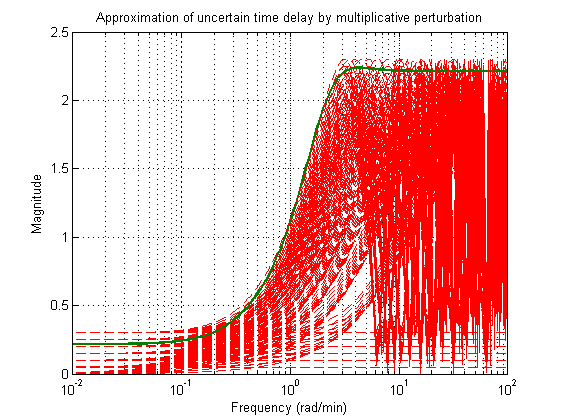
\includegraphics[width=75mm,keepaspectratio]{figures/2m06/unc_col_before.png}
	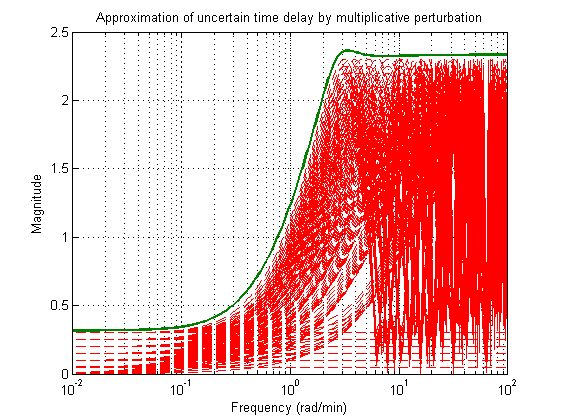
\includegraphics[width=75mm,keepaspectratio]{figures/2m06/unc_col_after.png}
	\caption{Új súlyozó függvény felvétele}
	\label{fig:Unc}
\end{figure}



\begin{figure}[!ht]
	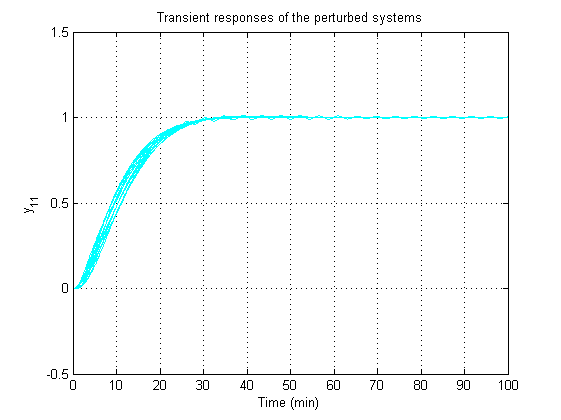
\includegraphics[width=75mm,keepaspectratio]{figures/2m06/prt_new_1_.png}
	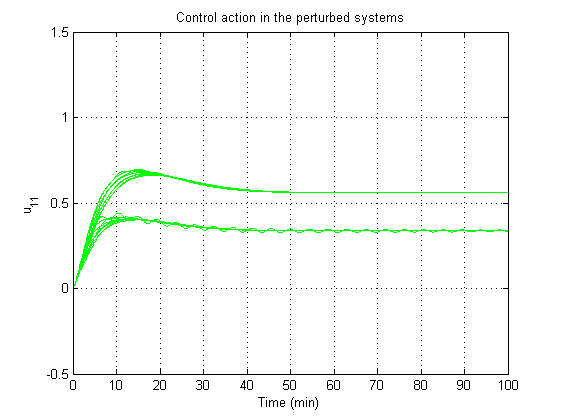
\includegraphics[width=75mm,keepaspectratio]{figures/2m06/prt_new_3_.png}
	\caption{Az új szabályzó viselkedése a kibővített bizonytalansági feltételek mellett}
	\label{fig:PrtNew}
\end{figure}




